\subsection{More Entropy for Login Keys}

\paragraph{Problem:}
Generally, neither the username nor the password provides good entropy.
The only rule imposed on the password is that it should have a minimum length of 8 characters.
Therefore, weak passwords such as \texttt{password} are accepted.

\paragraph{Consequences:}
We use \texttt{Scrypt(password, username + InstanceSalt)} to generate the login keys (master keys).
Since these master keys are not generated from a good source of randomness, attackers can gain access to all documents of users with weak passwords.

A side consequence is that the probability to register a new account with the same \texttt{username} and \texttt{password} combination is not negligible. If this happens, then users without bad intentions get access to a third person's drive.

\paragraph{Suggestions:}
Use password strength estimation such as \texttt{zxvbn-ts}~\cite{Wheeler2016,MrWook2022} which rates the password strength on a score from 0 to 4 and provides, guessing times, indicators what makes the password weak and how it can be improved (see \cref{fig:zxvbn}).
We may display the password strength estimation and/or require a minimum score.


\begin{figure}[t]
  \centering
  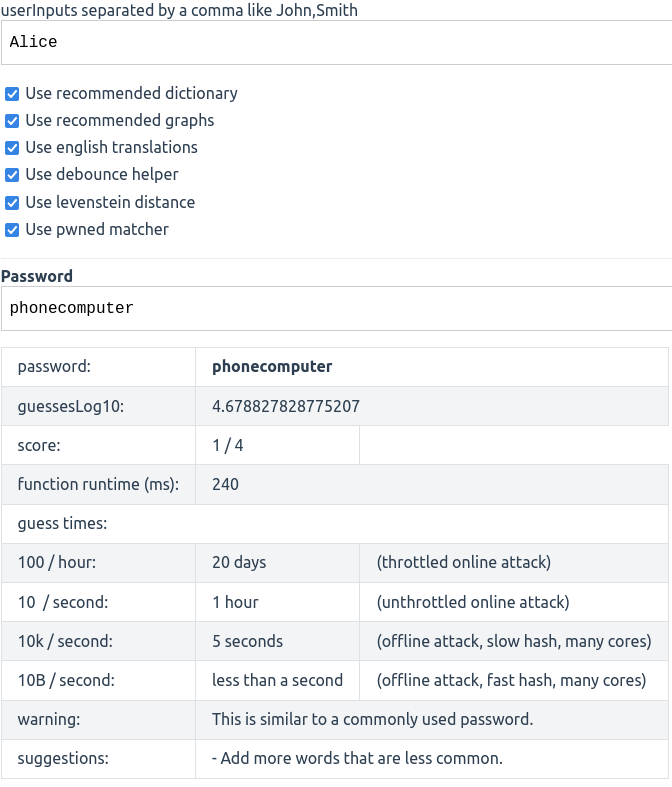
\includegraphics[width=0.55\columnwidth]{images/zxvbn.png}
  \caption{The library \texttt{zxvbn-ts} provides a score, guess times, warnings, and suggestions.}
  \label{fig:zxvbn}
\end{figure}

\paragraph{Drawbacks:} Users are annoyed by password requirements.
